\section{Resultados}

Para analisar a efetividade desse modelo, vamos analisar sob a ótica os critérios de avaliação, definidos na \secref{sec:success_metrics}.

\subsection{Corretude das previsões}

Para cada um dos valores de $LAG$, definidos na \secref{sec:lstm-metodology}, todas as previsões realizadas tenderam a "repetir" as sequências de áudio de entrada. Comparando os sinais digitais do arquivo de teste e os gerados na previsão, ilustrados na \figref{fig:lstm-repetition-results}, é possível notar que, quando alinhado com a sequência real de teste, não há nenhuma correspondência. No entanto, ao compararmos com os dados de entrada, isto é, o que construímos a lista $Z$, é possível notar uma clara semelhança. O formato da onda sonora foi mantido, diferindo apenas por sua amplitude.

Ademais, os áudios previstos soaram distorcidos, consequência das diferenças de amplitude encontradas nos sinais digitais da previsão contra a sequência de entrada.

Esses resultados foram observados em todas as janelas de entrada, tanto para os valores de $LAG$ 50 ms e 100 ms.

\begin{figure}
     \centering
     \begin{subfigure}[b]{0.49\textwidth}
         \centering
         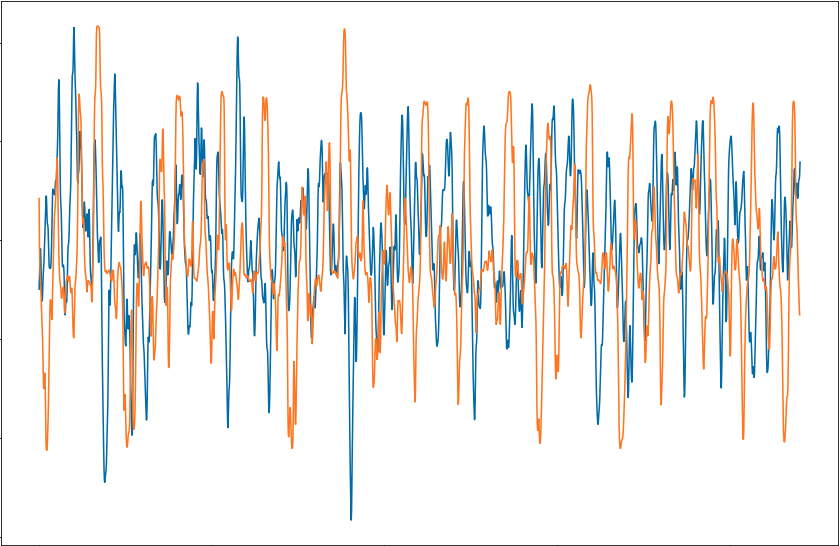
\includegraphics[width=\textwidth]{images/lstm-after.png}
         \caption{Previsão alinhada com a sequência real de teste.}
         \label{fig:y equals x}
     \end{subfigure}
     \hfill
     \begin{subfigure}[b]{0.49\textwidth}
         \centering
         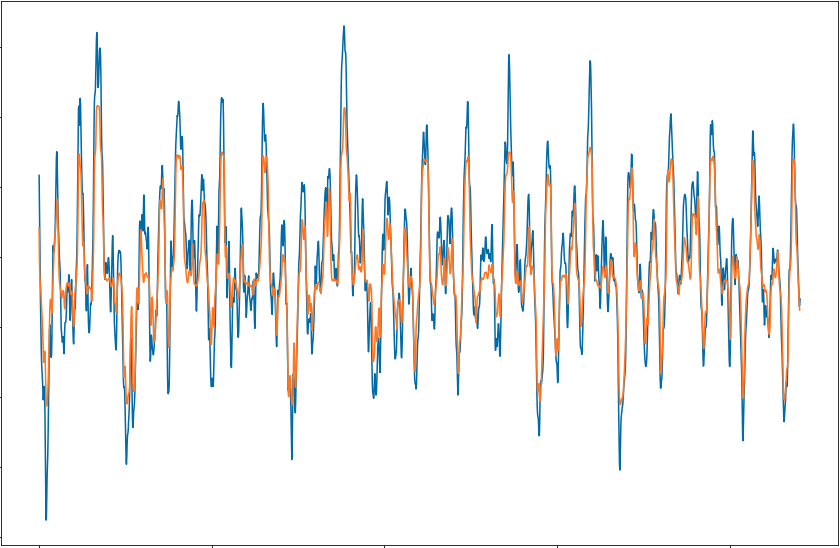
\includegraphics[width=\textwidth]{images/lstm-before.png}
         \caption{Previsão alinhada com a sequência de entrada.}
         \label{fig:three sin x}
     \end{subfigure}
        \caption{Comparação entre as sequências digitais geradas na previsão de uma das listas $Z$, em laranja, com (a) a sequência real de teste e (b) a sequência de entrada, ambas em azul, para o valor $LAG = 50 ms$.}
        \label{fig:lstm-repetition-results}
\end{figure}

Caso aplicássemos esse modelo em uma aplicação real, efetivamente estaríamos repetindo os dados transmitidos e, como discutido no \chapref{chap:solution_propositon}, retornaremos ao problema que as soluções \textit{delay-based} enfrentam. Portanto, não podemos atestar a corretude das previsões para o modelo preditivo gerador de novas sequências.

\subsection{Tempo de geração de previsões}

Na \tabref{tab:lstm-time-results}, podemos observar as médias de tempo para gerar as previsões para cada valor de $LAG$ testado, assim com o tempo médio de treinamento. É notável que, para nenhum dos dois valores, o tempo de previsão foi menor que o tempo da janela de previsão. Dessa forma, podemos afirmar que este modelo preditivo, como foi implementado, não satisfaz a métrica de sucesso para o tempo de previsão.

Ademais, vale notar que, apesar de não ser uma métrica de sucesso, que o tempo médio de treinamento foi relativamente alto, além de depender do valor de $LAG$.

\begin{table}[ht!]
    \centering
    \begin{tabular}{|c||c|c|}
        \hline
        
        Valor de LAG & Média de tempo de previsão & Média de tempo de treinamento por epoch \\
        
        \hline
        \hline
        
        50 ms & 150 ms & 55 s  \\ 
        \hline
        
        100 ms & 380 ms & 127 s \\ 
        \hline
    \end{tabular}
    \caption{Tabela comparando os tempos médios para gerar as previsões e para treinar os modelos para os valores 50 ms e 100 ms de simulação de latência da Internet.}
    \label{tab:lstm-time-results}
\end{table}
